\section{Procédés de fabrication des MID}
Il existe actuellement 2 méthodes de production de \textsc{mid} sur le marché :
le \emph{Laser Direct Structuring} et le \emph{Two-shot molding}. Le premier est
de loin le plus répandu (environ 80\% du marché selon \cite{mid-2011}), car moins
cher et plus adapté aux petites séries, tandis que le second est utilisé lorsque
la géométrie de la pièce ne permet pas l'usage du \textsc{lds}.

\subsection{Laser Direct Structuring}
\begin{figure}[h]
    \begin{center}
        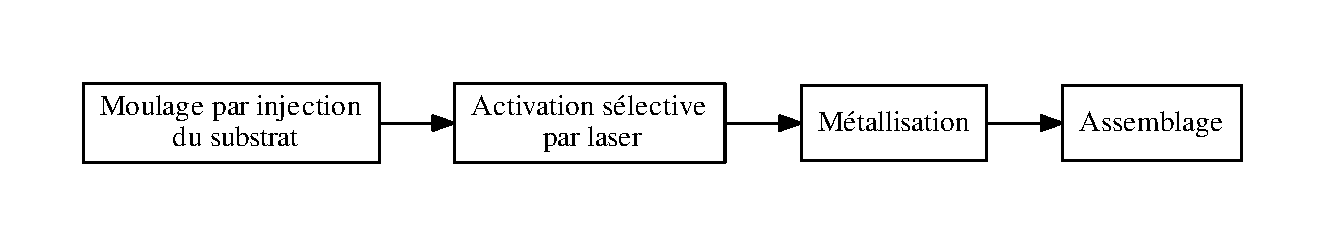
\includegraphics[width=\textwidth]{images/lds_process}
        \caption{Vue d'ensemble du processus \emph{Laser Direct Structuring}}\label{fig:lds-process}
    \end{center}
\end{figure}
Le \textsc{lds} est un procédé relativement récent, ayant été introduit sur le
marché en 2006. Par conséquent, c'est une technologie brevetée de LPKF Lasers \&
Electronics AG en Allemagne. Leur site web\footnote{\url{www.lpkf.com}} est donc
une excellente source d'informations pour la conception de pièces utilisant
le \textsc{lds-mid}.

\subsubsection{Principe de base du procédé}
Le principe général du procédé est visible à la fig. \ref{fig:lds-process}. On
retrouve donc, dans l'ordre :

\begin{description}
    \item[Injection] La pièce esLa pièce est d'abord moulée par un procédé
        d'injection standard. Le détail de cette étape sort du cadre de
        ce séminaire. On se référera à celui sur l'injection plastique. 
    \item[Activation] Le polymère ayant servi pour l'injection de la pièce a
        préalablement été
        dopé avec un composant organométallique qui est activé par le laser en
        suivant le tracé des pistes voulues. Une réaction physique décompose
        alors ce dopant entre partie métallique et partie organique.
        Les lasers utilisés sont typiquement des lasers infra-rouges d'une
    \item[Métallisation] L'étape de métallisation commence par une étape de
        nettoyage, afin de faciliter l'accrochage. Les pistes sont ensuites
        construites par dépose de fine couches (environ \SI{5}{\micro\meter}).
        Finalement, un traitement de surface contre l'oxydation est appliqué. Ce
        traitement consiste généralement en une couche de nickel suivi d'une
        couche d'or, mais des traitements spécifiques, à base d'étain ou
        d'argent sont également possibles.
    \item[Assemblage] Les composants électriques annexes (boutons, connecteurs,
        etc\ldots) sont soudés sur le \textsc{mid}. Pendant le prototypage cette
        étape est souvent faite à la main, avec un fer à souder. Pour la
        production, si le polymère a une température de fusion suffisament
        élevée, l'assemblage par \emph{reflow soldering} est possible. 
\end{description}

\subsubsection{Métallisation}
L'étape de métallisation est celle qui va déposer les pistes sur le poylmére à
proprement parler.
Afin de garantir le bon fonctionnement de cette étape, un rinçage de la pièce
entre chaque bains est effectué, ainsi qu'un séchage à chaud après le dernier
bain, afin d'enlever toute trace sur la pièce finale.

Le premier bain de cuivre se fait sans électrolyse, vu qu'aucune piste
conductrice n'existe pour le moment. Dans ce bain, du cuivre va croître autour
des atomes de métail présent à la surface du polymère et se liera au
microcavités résultant de l'activation laser. L'épaisseur maximum atteignable
lors de ce premier bain est de 5 à 8 \si{\micro\meter}.

Dans les applications à fort courants, une grande épaisseur de cuivre est
souhaitée. Pour y parvernir, on peut, après le premier bain, faire une dépose
éléctrolytique du cuivre. Pour cela, il faut que toute les pistes soit
connectées entre elles en un point. Si ce n'était pas le cas, il faudrait
connecter les pistes une à une à l'éléctrode, ce qui serait long et donc
coûteux. Le point de connexion est généralement placé sur une partie séparable
mécaniquement qui est enlevée après la métallisation.

Une fois ce premier bain terminé, une couche de protection contre l'oxydation
est appliquée. En effet une oxydation de la couche de cuivre ruinerait les
proprietés électriques du circuit.
Cette couche est généralement composée d'une couche de nickel
suivie d'une couche d'or. Le rôle de la couche d'or est d'empêcher l'oxydation
de la couche de cuivre. La couche de nickel sert à empêcher le cuivre de
diffuser dans l'or, ce qui détruirait la protection anti-oxydation.
